\subsection*{Карбонилы 6 и 10 групп}

Карбонильные лиганды очень похожи на цианидные, однако в их случае ориентироваться на ТКП не рекомендуется, ведь $CO$, как и металл, не заряжен. 

\subsubsection*{VI гр.}

\begin{figure}[H]
\centering
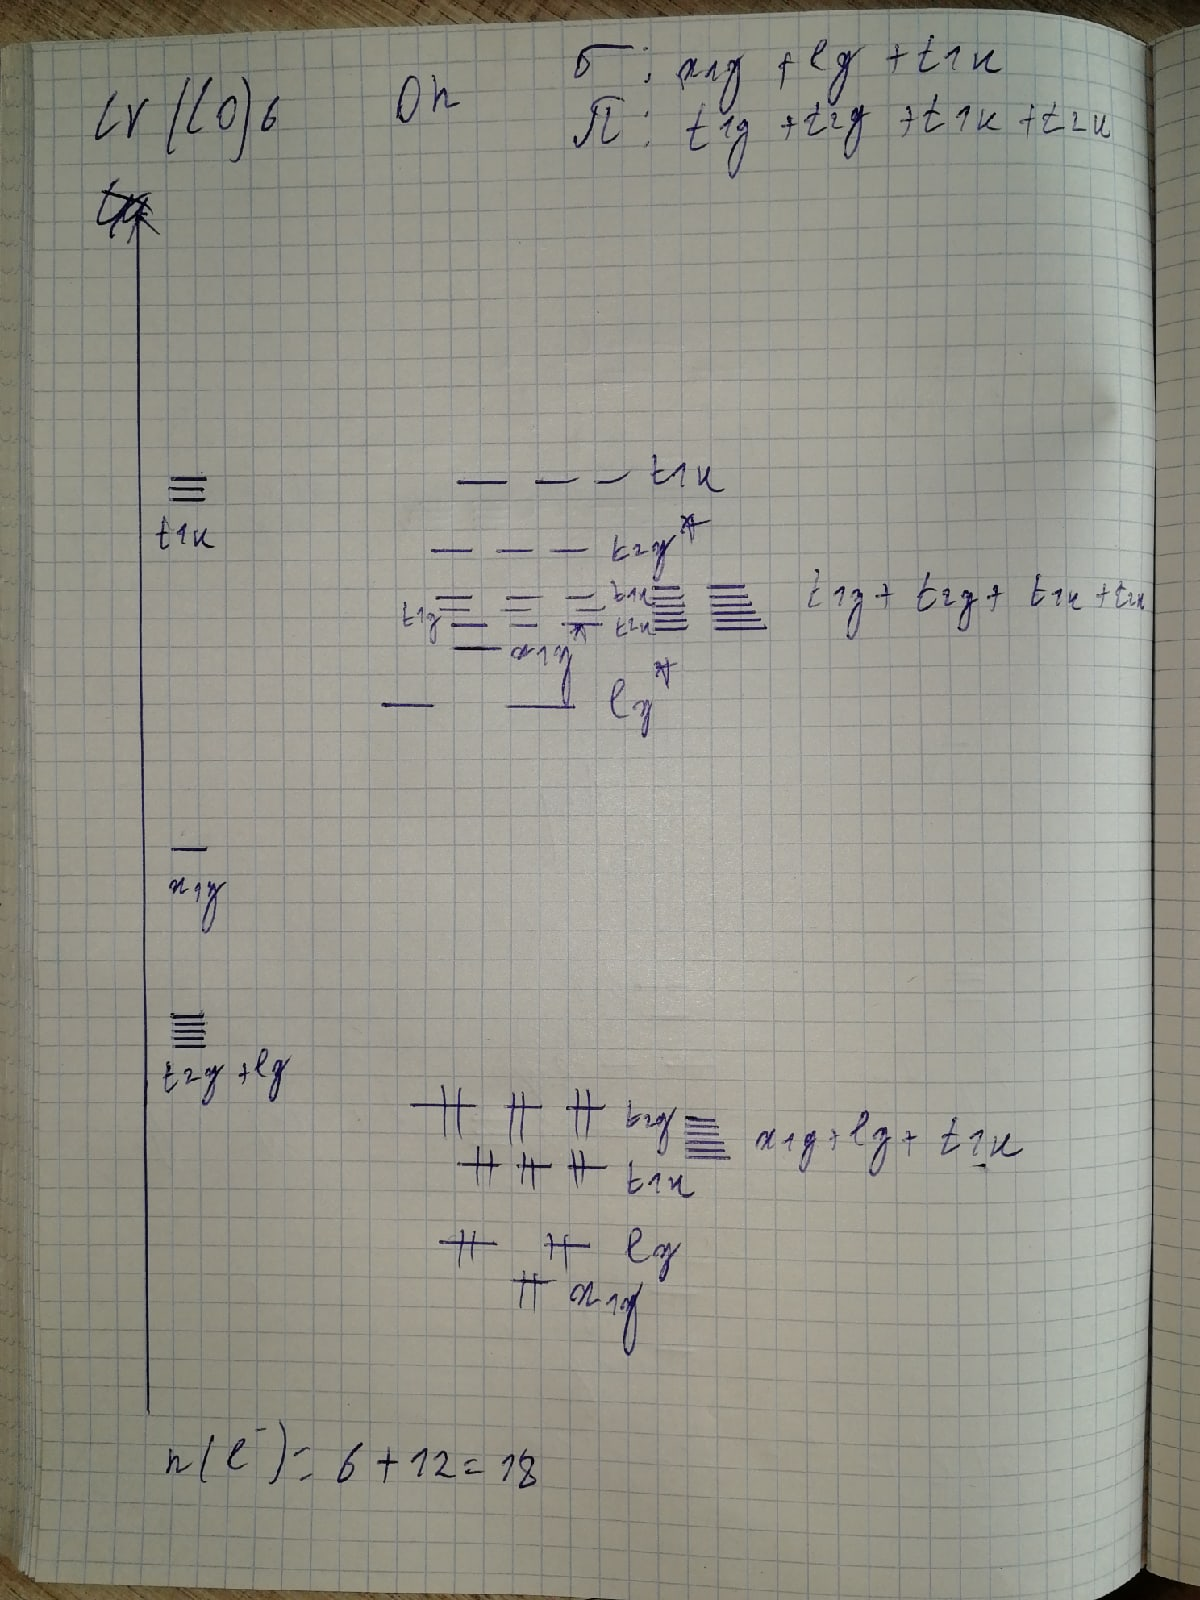
\includegraphics[scale=.300]{images/carboniles.jpg}
\end{figure}
Строение октаэдрическое. Здесь выполняется правильно Сиджвика. Заполнены все связывающие орбитали, комплекс довольно прочный. Диамагнитен, окрашивания почти не видно. ПС=6, КС=1.

Если идти к молибдену и вольфраму, то там орбитали металла ещё выше. Связывание с $e_g$ и $a_{1g}$ ухудшается, прочность комплексов падает.

\begin{figure}[H]
\centering
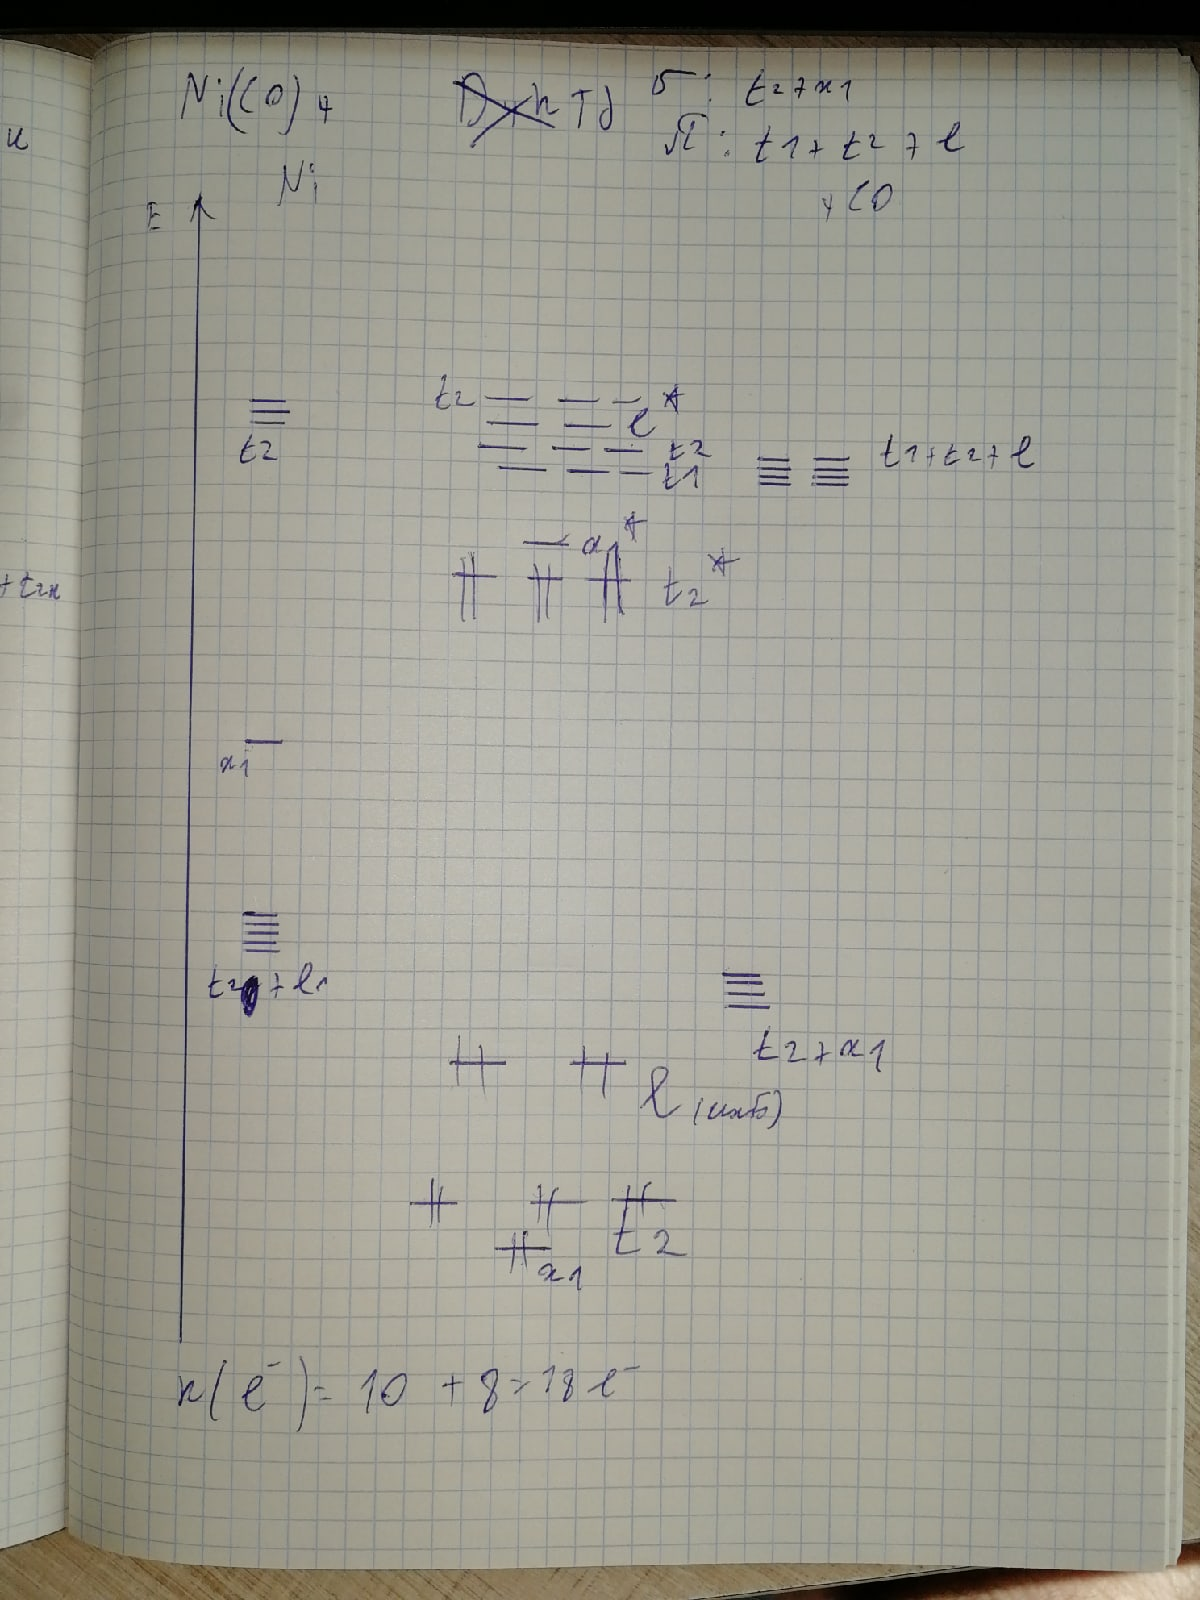
\includegraphics[scale=.300]{images/carboniles2.jpg}
\end{figure}

\subsubsection*{X гр.}
Рассмотрим $Ni(CO)_4$, который имеет форму тетраэдра:


Здесь ситуация интереснее, т.к. заполнена и часть разрыхляющих орбиталей, что подтверждается меньшей устойчивостью этого комплекса. Он диамагнитен и бесцветен, т.к. орбиталь $a_1^*$ сильно выше, чем $t_2^*$(просто масштаб хреновый).
Для платины и палладия таких карбонилов не зафиксировано, т.к. они не склонны к отдаче электронов на $\pi^*$-орбитали $CO$.